% Chapter 4 -- Rubric: PO3 (3.3, 3.4), PO5 (5.1)
\chapter{System Design and Implementation}
\label{ch:design}

% \section{Functional Design and Sub-problem Partitioning}
% \label{sec:architecture}
% \begin{figure}[htbp]
%   \centering
%   \figplaceholder{Architecture diagram}
%   \caption{System architecture}
%   \label{fig:architecture}
% \end{figure}
% \guidance{Partition the problem into sub-problems or modules; explain each one's
% responsibility and how they interact. Show where the standards and codes of
% practice from \Cref{sec:standards} and any health, safety, or environmental
% considerations shaped the design.}

\section{Functional Design and Sub-problem Partitioning}
\label{sec:architecture}

The system was decomposed along two independent axes. The first is a separation
by execution context where work that must answer a user within the lifetime of
an HTTP request is handled by one process, while work that is long-running,
retryable or scheduled is handled by another. The second is a separation by
domain concern where the logic for talking to an external tool, for computing a
score, for queueing a job and for encrypting a credential are each isolated
behind an interface, so that none of them depends on the details of the others.

\Cref{fig:architecture} shows the resulting structure.

\begin{figure}[htbp]
\centering
\begin{tikzpicture}[
  font=\small,
  proc/.style={draw, thick, rounded corners=3pt, align=left, inner sep=2.2mm,
               text width=36mm},
  infra/.style={draw, rounded corners=2pt, align=center, inner sep=2mm},
  chip/.style={draw, rounded corners=1pt, align=center, text width=21mm,
               inner sep=1.3mm, font=\scriptsize},
  ext/.style={draw, dashed, rounded corners=2pt, align=center, inner sep=2mm},
  band/.style={draw, dashed, rounded corners=3pt, inner sep=2.4mm},
  arr/.style={-{Stealth[length=2mm]}, thick},
  tag/.style={font=\scriptsize, fill=white, inner sep=1pt}
]

%% ---- processes ----
\node[proc] (api) at (0,0) {\textbf{API process}\\[2pt]
  {\scriptsize HTTP routing and validation}\\
  {\scriptsize Authentication and sessions}\\
  {\scriptsize Tenancy and authorisation}\\
  {\scriptsize Project, survey, action services}\\
  {\scriptsize Progress streaming (SSE)}};

\node[infra, text width=19mm, right=15mm of api] (redis) {\textbf{Redis}\\[1pt]
  {\scriptsize Job queues}\\
  {\scriptsize Pub/sub}\\
  {\scriptsize Sessions}};

\node[proc, right=15mm of redis] (worker) {\textbf{Worker process}\\[2pt]
  {\scriptsize Sync processor}\\
  {\scriptsize Scheduled sync fan-out}\\
  {\scriptsize Survey distribution and send}\\
  {\scriptsize Survey insight analysis}\\
  {\scriptsize Action embedding}};

%% ---- client ----
\node[infra, text width=36mm, above=12mm of api] (client) {\textbf{Web client}\\[1pt]
  {\scriptsize React single-page application}};

%% ---- shared domain libraries ----
\node[chip, below=15mm of api.south west, anchor=north west] (p1)
  {Persistence\\layer};
\node[chip, right=2.5mm of p1] (p2) {Security\\(crypto)};
\node[chip, right=2.5mm of p2] (p3) {Risk\\engine};
\node[chip, right=2.5mm of p3] (p4) {Connector\\interface};
\node[chip, right=2.5mm of p4] (p5) {AI, embeddings,\\notifications};

\begin{scope}[on background layer]
  \node[band, fit=(p1)(p5),
        label={[font=\scriptsize]above left:Shared domain libraries}] (libs) {};
\end{scope}

%% ---- infrastructure and external systems ----
\node[infra, text width=42mm] (db)
  at ($(p1.south)!0.2!(p2.south) + (0,-20mm)$)
  {\textbf{PostgreSQL (Supabase)}\\[1pt]
   {\scriptsize snapshots, scores, surveys, actions}};

\node[ext, text width=40mm] (extsys)
  at ($(p4.south)!-0.5!(p5.south) + (0,-20mm)$)
  {\textbf{External systems}\\[1pt]
   {\scriptsize Tools: VCS, Project management, CI/CD, Code quality}};

\node[ext, text width=40mm] (fxtsys)
  at ($(p4.south)!1.5!(p5.south) + (0,-20mm)$)
  {\textbf{External systems}\\[1pt]
   {\scriptsize AI, Email}};

%% ---- flows ----
\draw[arr] (client) -- node[tag, right] {REST} (api);
\draw[arr] (api.west) to[out=170, in=190, looseness=2]
  node[tag, left] {SSE} (client.west);

\draw[arr] (api) -- node[tag, above] {enqueue} (redis);
\draw[arr] (redis) -- node[tag, above] {dequeue} (worker);
\draw[arr] (worker.south west) to[out=215, in=325]
  node[tag, below] {progress} (redis.south east);

\draw[arr] (api.south) -- (api.south |- libs.north);
\draw[arr] (worker.south) -- (worker.south |- libs.north);

\draw[arr] (p1.south) -- (db.north);
\draw[arr] (p4.south) -- (extsys.north);
\draw[arr] (p5.south) -- (fxtsys.north);
\end{tikzpicture}
\caption{System architecture. The API process serves the client synchronously and
the worker performs all long-running and scheduled work; Redis carries both the
job queues between them and the progress events flowing back. Both processes draw
on the same domain libraries, which are the only components that contact the
database or external systems.}
\label{fig:architecture}
\end{figure}


\subsection{Rationale for the Partition}
\label{subsec:partition-rationale}

Splitting the API and worker into separate processes follows from the nature of
the work. A single synchronisation queries four external APIs, some with
pagination over hundreds of records, and can run for minutes. Performing that
inside a request would hold the connection open far beyond any reasonable
timeout, and a failure part-way through would leave the user with an error and no
record of the partial work. Moving it to a worker allows the request to return
immediately with an acknowledgement, and allows the work itself to be retried,
prioritised and rate-limited independently of any user waiting on it (NFR-11,
NFR-16).

That separation creates a problem of its own: the worker performs the work, but
only the API process holds a connection to the user's browser, so the worker
cannot report progress directly. Redis resolves this by carrying both directions
of the exchange. It holds the job queues through which the API hands work to the
worker, and it carries a publish/subscribe channel per synchronisation session
through which the worker reports progress back. The API subscribes to that
channel and relays each event to the browser over Server-Sent Events. The final
completion event is additionally retained in Redis for a limited period, so that a
client which reloads the page after a synchronisation has finished still receives
its outcome rather than waiting on a channel that will never speak again
(FR-17).

\subsection{Module Responsibilities}
\label{subsec:module-responsibilities}

\begin{longtable}{
  >{\raggedright\arraybackslash}p{0.24\textwidth}
  >{\raggedright\arraybackslash}p{0.34\textwidth}
  >{\raggedright\arraybackslash}p{0.28\textwidth}
}
\caption{Modules, their responsibilities and principal interactions}
\label{tab:modules}\\
\toprule
\textbf{Module} & \textbf{Responsibility} & \textbf{Interacts with} \\
\midrule
\endfirsthead
\toprule
\textbf{Module} & \textbf{Responsibility} & \textbf{Interacts with} \\
\midrule
\endhead
\bottomrule
\endlastfoot
Web client & Presents the portfolio, dashboards, settings and survey interfaces;
consumes the progress stream & API process \\
\addlinespace
HTTP interface layer & Routes requests, validates input, maps domain errors to status
codes & All API-side services \\
\addlinespace
Authentication and session management & Verifies credentials, issues and revokes
sessions, manages verification, invitation and reset tokens & Redis session store,
user data access \\
\addlinespace
Authorisation and tenancy & Restricts every access to the caller's company, and
further to assigned projects for non-administrators & All API-side services \\
\addlinespace
Project and workspace services & Repository import, tool integration configuration,
member management & Data access, connector repository listing \\
\addlinespace
Progress streaming & Subscribes to a session's event channel and relays events to the
browser & Redis pub/sub \\
\addlinespace
Queue abstraction & Declares the job queues, their retry, priority and retention
policies, and the scheduler & API process, worker process, Redis \\
\addlinespace
Sync processor & Orchestrates one synchronisation: fetch, persist, score, report &
Connectors, persistence, risk engine, event store \\
\addlinespace
Scheduled sync fan-out & Expands a scheduler tick into one queued job per project,
staggered by shared credential & Queue abstraction, project data access \\
\addlinespace
Survey processors & Assign monthly pulses, generate questions, dispatch links,
analyse responses on close & AI client, notification clients, survey data access \\
\addlinespace
Connector interface & Presents one interface per tool category; each provider
implementation converts a vendor API into a normalised metric object & Worker
process, external tool APIs \\
\addlinespace
Risk engine & Converts a normalised metric set into the seven health scores, with
weights and null handling & Sync processor, survey health context \\
\addlinespace
AI client abstraction & Question generation, question scoring and response analysis
behind a provider-independent interface & Survey processors \\
\addlinespace
Embedding and search & Produces and stores action vectors; performs semantic
retrieval and reranking & Action services, worker process \\
\addlinespace
Security module & Credential encryption at rest and survey link sealing & Data access
layer, survey dispatch \\
\addlinespace
Notification clients & Delivers survey links to team channels and transactional email
& Survey processors \\
\addlinespace
Persistence layer & All database access, with encryption and decryption applied at
this boundary & Every module above \\
\end{longtable}

Three of these boundaries carry most of the design's extensibility, and are worth
stating explicitly.

The \textbf{connector interface} is what satisfies O-07 and NFR-21. Each
provider implements a single method returning a normalised metric object, and a
registry maps a tool name to its implementation. Nothing downstream of that
interface, not the sync processor, not the persistence layer, not the risk
engine, contains any provider-specific logic. Adding a new version-control
provider is therefore the addition of one class and one registry entry.

The \textbf{risk engine} isolates scoring behind a similar boundary. Each of the
seven dimensions is an independent strategy selected by an enumeration, and every
strategy is built from the same shared set of normalisation functions and a
common null-aware weighting routine. A dimension's rules can be changed, or a
dimension added, without touching ingestion or presentation which is a property that
was exercised in practice when the scoring model was revised, as described in
\Cref{sec:detailed-design}.

The \textbf{persistence layer} is the single point at which credential encryption
is applied. Encryption occurs on write and decryption on read, both inside the
data-access functions, so that every module above this boundary operates on
plaintext and none of them can accidentally persist an unencrypted credential.

\subsection{Interaction: The Synchronisation Path}
\label{subsec:interaction-sync}

The synchronisation flow exercises most of the system and illustrates how the
modules cooperate. A request arrives at the HTTP layer, which validates it and
confirms through the authorisation module that the caller may act on the named
project. The project service resolves the configured integrations, decrypting
each credential at the persistence boundary and resolving the version-control
token from the owning workspace where the project does not carry its own. The
queue abstraction enqueues a job carrying the project, the tool list and the
session identifier, and the request returns an acknowledgement.

The worker dequeues the job and creates one snapshot record for the run. It then
fetches from the configured tools concurrently, subject to a concurrency bound
(NFR-15), publishing a progress event as each tool begins and finishes. Each
tool's normalised output is written against the shared snapshot. A tool that
fails is recorded as failed and the run continues (FR-19, NFR-10). Once
persistence is complete, the risk engine computes the seven scores from whatever
metrics the snapshot actually contains, redistributing the weight of absent
inputs (FR-22), and the scores are stored against the snapshot. A completion
event is published and retained. Throughout, the API process has been relaying
each published event to the browser, which updates per-tool status in place.

\subsection{Influence of Standards and Codes of Practice}
\label{subsec:standards-in-design}

The obligations established in \Cref{sec:standards} were not applied as a review
performed after construction; several of them determined where module boundaries
were drawn in the first place. \Cref{tab:standards-design} records where each
one is realised in the structure.

\begin{longtable}{
  >{\raggedright\arraybackslash}p{0.26\textwidth}
  >{\raggedright\arraybackslash}p{0.60\textwidth}
}
\caption{Where the standards of \Cref{sec:standards} shaped the design}
\label{tab:standards-design}\\
\toprule
\textbf{Obligation} & \textbf{Effect on the design} \\
\midrule
\endfirsthead
\toprule
\textbf{Obligation} & \textbf{Effect on the design} \\
\midrule
\endhead
\bottomrule
\endlastfoot
Access control (OWASP A01) & Tenancy scoping is applied inside the persistence layer
rather than in individual handlers, so that a query cannot omit it by oversight. Role
and project-membership checks sit in the service layer, above it \\
\addlinespace
Cryptographic protection (OWASP A02) & All cryptography is confined to a single
security module, and applied at the persistence boundary. No other module performs
encryption, which keeps the algorithm, key handling and versioning in one auditable
place \\
\addlinespace
Injection resistance (OWASP A03) & A single parameterised data-access client is the
only route to the database; no module composes SQL. One shared helper sanitises
user-supplied search terms, and one escapes values placed into outgoing email \\
\addlinespace
Abuse resistance (OWASP A04) & Rate limiting is applied as middleware at the router
handling unauthenticated requests. Dispatch quotas and recipient cooldowns are
enforced inside the survey dispatch module, not at the call sites that invoke it \\
\addlinespace
Respondent anonymity (NFR-07) & Enforced structurally rather than procedurally: the
survey response table carries no foreign key to a user, so no query can reconstruct
the association. The design places the guarantee in the schema, where application
code cannot circumvent it \\
\addlinespace
Data minimisation & The AI client abstraction is the only module permitted to
transmit data externally for analysis, and the prompt-construction layer strips
personal names and work-item identifiers before transmission, giving a single
chokepoint to audit \\
\addlinespace
Temporal correctness (ISO 8601, RFC 3339) & Timestamp parsing and formatting are
centralised in a shared utility, and the database columns were migrated to zone-aware
types so that instants are unambiguous regardless of the reader's locale \\
\addlinespace
Accessibility (WCAG 2.1 AA) & Interactive elements in the client are built from
shared components that carry role, focus and keyboard behaviour by default, so that
accessibility properties are inherited rather than reapplied per screen \\
\end{longtable}

\subsection{Health, Safety and Environmental Considerations}
\label{subsec:hse-design}

The system performs no physical actuation and controls no equipment, so the
safety considerations that govern cyber-physical systems do not arise. Two
related considerations do apply, and both influenced the design.

The first concerns \textbf{occupational wellbeing}. The system measures the work
of identifiable people, and a monitoring tool of this kind can readily become an
instrument of individual performance assessment with predictable effects on
the behaviour of those measured. Three design decisions deliberately foreclose
that use. Metrics are aggregated to the project level and no per-developer view
exists anywhere in the interface, despite the underlying data making one
technically feasible. Qualitative feedback is anonymous by schema construction,
as described above, so that candour carries no personal risk. And survey dispatch
is bounded by per-project quotas and per-recipient cooldowns, so that
participation does not itself become a burden. These constraints resolve the
conflict between managerial visibility and developer psychological safety
identified in \Cref{subsec:conflicts}, and they are properties of the design rather
than matters of policy.

The second concerns \textbf{resource consumption}. Two choices reduce it
materially. Collection is scheduled rather than continuous, so the system issues
a bounded number of external requests per project per day instead of polling,
and projects sharing a credential are staggered, which flattens the load profile
rather than concentrating it. Both were adopted primarily to respect third-party
rate limits and free-tier quotas, but their effect on energy and network
consumption is the same. The resources the deployment consumes are quantified in
\Cref{sec:deployment}, and their environmental impact assessed in
\Cref{sec:sustainability}.

% \section{Design Refinement and Simulation}
% \label{sec:detailed-design}
% \guidance{Present the detailed design using the views that fit the project (ERD,
% class, sequence, DFD, API, wireframes, circuit, model). Include any design
% calculations or estimates made (e.g. expected load or storage), the
% analyses, prototypes, or simulations used to verify the design against the
% requirements, and how the design was refined to facilitate implementation.}


\section{Design Refinement and Simulation}
\label{sec:detailed-design}

This section presents the detailed design through the views that carry the most
information about this system such as the structure of the two extensible layers, the
data model, the synchronisation sequence, and the external interface. It then
records the storage and load estimates made during design, the means by which the
design was checked against its requirements, and the refinements made to the
design during implementation.

\subsection{Structure of the Connector and Scoring Layers}
\label{subsec:connector-scoring-structure}

\Cref{fig:connector-scoring} shows the internal structure of the two layers that
carry the system's extensibility, and the path by which data travels from one to
the other. External tool APIs are omitted here; they appear in
\Cref{fig:architecture}.

\begin{figure}[htbp]
\centering
\begin{tikzpicture}[
  font=\footnotesize,
  iface/.style={draw, rounded corners=1pt, align=center, text width=50mm,
                inner sep=1.6mm},
  cls/.style={draw, align=left, text width=32mm, inner sep=1.6mm},
  ghost/.style={draw, dashed, align=left, text width=32mm, inner sep=1.6mm},
  store/.style={draw, rounded corners=2pt, align=center, text width=32mm,
                inner sep=1.8mm},
  arr/.style={-{Stealth[length=2mm]}, thick},
  real/.style={-{Triangle[open, length=2.6mm]}, dashed, thin},
  % step/.style={font=\scriptsize\bfseries, fill=white, inner sep=1pt}
  flowstep/.style={font=\scriptsize\bfseries, fill=white, inner sep=1pt}
]


%% ---------- centre: worker and store ----------
\node[store] (proc) at (0mm,0mm) {\textbf{Sync processor}\\[1pt]
  {\scriptsize worker process}};
\node[store, text width=34mm] (snap) at (0mm,-52mm)
  {\textbf{Project snapshot}\\[1pt]
   {\scriptsize normalised metrics per tool}\\
   {\scriptsize + seven scores}};

%% ---------- left: connector layer ----------
\node[iface] (reg) at (-48mm,0mm) {\texttt{createConnector(tool)}\\[1pt]
  {\scriptsize registry: name $\rightarrow$ implementation}};
\node[iface] (iface) at (-48mm,-30mm)
  {{\scriptsize\itshape interface}\\ \texttt{IConnector}\\[1pt]
   {\scriptsize \texttt{getData()}}};
\node[cls] (impl) at (-48mm,-60mm) {\textbf{Implemented}\\[1pt]
  {\scriptsize GitHubConnector (VCS)}\\
  {\scriptsize JiraConnector (PM)}\\
  {\scriptsize SonarQubeConnector (quality)}\\
  {\scriptsize GithubActionsConnector (CI/CD)}};
\node[ghost] (future) at (-48mm,-90mm) {\textbf{Further providers}\\[1pt]
  {\scriptsize implement the interface, register once}};

%% ---------- right: scoring layer ----------
\node[store] (rcs) at (52mm,-52mm) {\textbf{Risk calculation service}\\[1pt]
  {\scriptsize shapes stored metrics into typed inputs}};
\node[iface] (engine) at (52mm,-80mm) {\texttt{RiskEngine}\\[1pt]
  {\scriptsize dispatch by \texttt{RiskType}}};
\node[iface] (rcalc) at (52mm,-100mm)
  {{\scriptsize\itshape interface}\\ \texttt{RiskCalculator<TMetrics>}};
\node[cls] (strat) at (52mm,-130mm) {\textbf{Seven strategies}\\[1pt]
  {\scriptsize Security, Reliability, Maintainability,}\\
  {\scriptsize CI/CD, Team Health, Engineering}\\
  {\scriptsize Process, Planning and Execution}};
\node[cls] (util) at (52mm,-160mm) {\textbf{Shared scoring functions}\\[1pt]
  {\scriptsize normalisers, null-aware weighting}};

%% ---------- realisation: orthogonal spine at x = -70mm ----------
\draw[real] (impl.west)   -- (-80mm,-60mm)  -- (-80mm,-30mm) -- (iface.west);
% \draw[real] (stub.west)   -- (-70mm,-90mm)  -- (-70mm,-30mm) -- (iface.west);
\draw[real] (future.west) -- (-80mm,-90mm) -- (-80mm,-30mm) -- (iface.west);
\draw[real] (strat.north) -- (rcalc.south);

%% ---------- flow ----------
\draw[arr] (proc.west) -- node[flowstep, above] {1} (reg.east);
\draw[arr] (reg.south) -- (iface.north);
\draw[arr] (iface.east) -- node[flowstep, above right] {2} (proc.south west);
\draw[arr] (proc.south) -- node[flowstep, right] {3} (snap.north);
\draw[arr] (snap.east) -- node[flowstep, above] {4} (rcs.west);
\draw[arr] (rcs.south) -- node[flowstep, right] {5} (engine.north);
\draw[arr] (engine.east) -- (80mm,-80mm) -- (80mm,-130mm) -- (strat.east);
\draw[arr] (strat.south) -- (util.north);
\draw[arr] (rcs.north west) to[bend left=30]
  node[flowstep, above] {6} (snap.north east);
\end{tikzpicture}

\caption{Structure of the connector and scoring layers. The worker depends only
on the \texttt{IConnector} interface, never on a specific provider (1--2);
normalised metrics are written to the snapshot (3) and read back from it for
scoring (4--6), so the two layers never reference each other directly.}
\label{fig:connector-scoring}
\end{figure}

\paragraph{The connector extension point.}
Every provider implementation satisfies one interface, \texttt{IConnector},
declaring a single method that returns a normalised metric object. A registry maps
each supported tool name to the function that constructs its implementation, and
the sync processor obtains a connector only through that registry. The
consequence is that the worker contains no reference to any specific provider, 
it names a tool, receives something satisfying the interface, and calls one method
on it. Provider-specific concerns, GitHub's separate REST and GraphQL rate
budgets, Jira's instance-specific custom field identifiers, SonarQube's paginated
measure history, are confined entirely within their own implementations.

Adding a provider therefore costs one class and one registry entry, with no
change to the sync processor, the persistence layer or the scoring engine. This
is what satisfies O-07 and NFR-21.

\paragraph{Decoupling of ingestion from scoring.}
The connector layer and the risk engine never communicate directly. The worker
writes each tool's normalised output to the project snapshot, and the risk
calculation service subsequently reads those stored metrics back out, shapes them
into the typed input object each strategy expects, and invokes the engine. The
snapshot is the integration point between ingestion and scoring.

This indirection is deliberate, and it buys three properties. Scoring becomes
reproducible. Since the inputs are stored rather than consumed in flight, a
score can be recomputed at any later time from the snapshot that produced it,
without contacting any external tool, which is how the per-metric score
breakdown of FR-26 is served months after the data was collected. Scoring also
becomes independently revisable. The weighting rules can change and be re-applied
to historical snapshots, because the raw evidence was retained. And a failure in
either layer is harmless to the other. A connector fault costs one tool's metrics for one
snapshot, while a scoring fault leaves the ingested data intact for later
recomputation.

\paragraph{The scoring extension point.}
The risk engine mirrors the connector layer's shape. Each of the seven dimensions
is an independent strategy implementing \texttt{RiskCalculator<TMetrics>},
generic in the metric type it consumes, and the engine dispatches to the
appropriate one by enumeration member. Each strategy declares its inputs as a
list of weighted signals and delegates the arithmetic to a shared set of
normalisation functions and a common null-aware weighting routine, so that the
behaviour on missing data (FR-22) is implemented once and identically for every
dimension rather than restated seven times.

A dimension's weights or thresholds can therefore be changed by editing one
strategy, and a dimension can be added by writing one class and one enumeration
member. That this holds in practice was demonstrated during development, when the
scoring model was restructured from six categories to seven, the change was
confined to the strategy layer and the score persistence schema, leaving
ingestion, the queue, the progress stream and the client untouched.


\subsection{Data Model}
\label{subsec:data-model}

The schema comprises seventeen tables, presented here in three related views:
tenancy and project structure (\Cref{fig:erd-tenancy}), metric capture and
scoring (\Cref{fig:erd-metrics}), and team engagement (\Cref{fig:erd-engagement}).
The \texttt{project} entity appears in all three, as it is the point on which
every other concern hangs.

\begin{figure}[htbp]
\centering
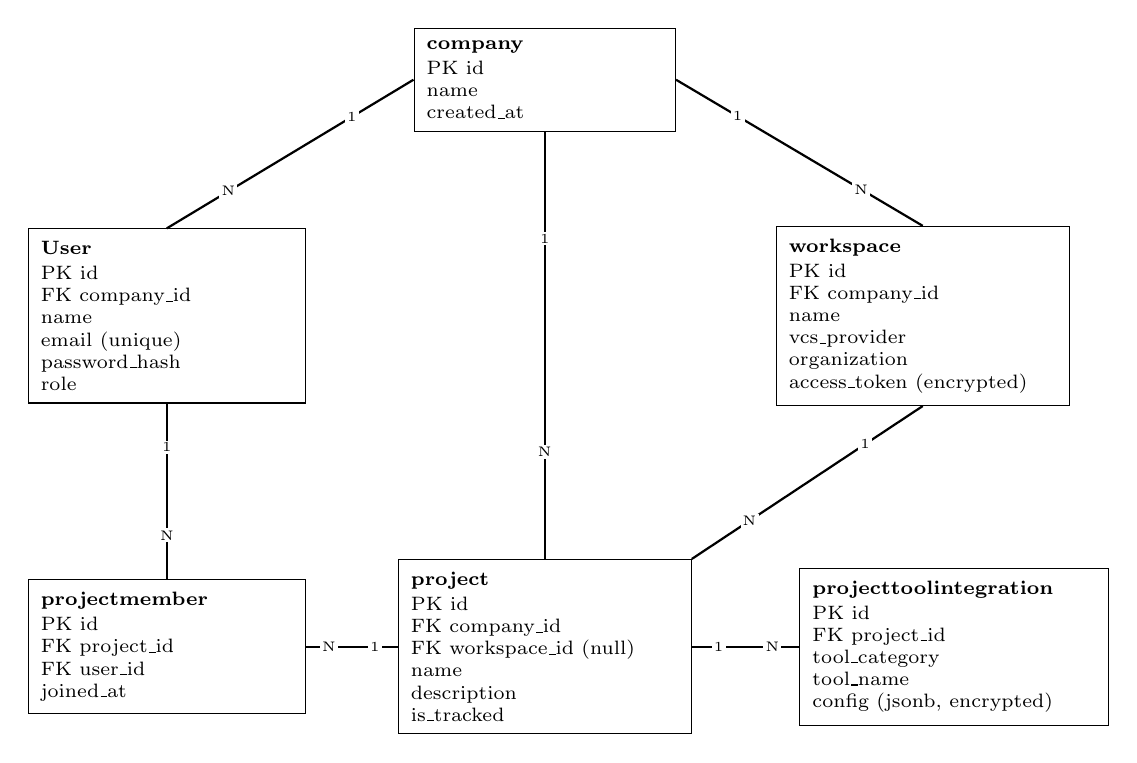
\begin{tikzpicture}[
  font=\scriptsize,
  ent/.style={draw, align=left, inner sep=1.6mm},
  rel/.style={thick},
  card/.style={font=\tiny, fill=white, inner sep=0.8pt}
]
\node[ent, text width=30mm] (co) at (0mm,0mm)
  {\textbf{company}\\[1pt] PK id\\ name\\ created\_at};

\node[ent, text width=32mm] (usr) at (-48mm,-30mm)
  {\textbf{User}\\[1pt] PK id\\ FK company\_id\\ name\\ email (unique)\\
   password\_hash\\ role};

\node[ent, text width=34mm] (ws) at (48mm,-30mm)
  {\textbf{workspace}\\[1pt] PK id\\ FK company\_id\\ name\\ vcs\_provider\\
   organization\\ access\_token (encrypted)};

\node[ent, text width=32mm] (pm) at (-48mm,-72mm)
  {\textbf{projectmember}\\[1pt] PK id\\ FK project\_id\\ FK user\_id\\ joined\_at};

\node[ent, text width=34mm] (proj) at (0mm,-72mm)
  {\textbf{project}\\[1pt] PK id\\ FK company\_id\\ FK workspace\_id (null)\\
   name\\ description\\ is\_tracked};

\node[ent, text width=36mm] (pti) at (52mm,-72mm)
  {\textbf{projecttoolintegration}\\[1pt] PK id\\ FK project\_id\\ tool\_category\\
   tool\_name\\ config (jsonb, encrypted)};

\draw[rel] (co.west) -- node[card, near start] {1} node[card, near end] {N}
(usr.north);
\draw[rel] (co.east) -- node[card, near start] {1} node[card, near end] {N}
(ws.north);
\draw[rel] (co.south) -- node[card, near start] {1} node[card, near end] {N}
(proj.north);
\draw[rel] (ws.south) -- node[card, near start] {1} node[card, near end] {N}
(proj.north east);
\draw[rel] (usr.south) -- node[card, near start] {1} node[card, near end] {N}
(pm.north);
\draw[rel] (proj.west) -- node[card, near start] {1} node[card, near end] {N}
(pm.east);
\draw[rel] (proj.east) -- node[card, near start] {1} node[card, near end] {N}
(pti.west);
\end{tikzpicture}
\caption{Tenancy and project structure. Every entity is owned by a company, which
is the tenancy boundary enforced on all data access.}
\label{fig:erd-tenancy}
\end{figure}

\begin{figure}[htbp]
\centering
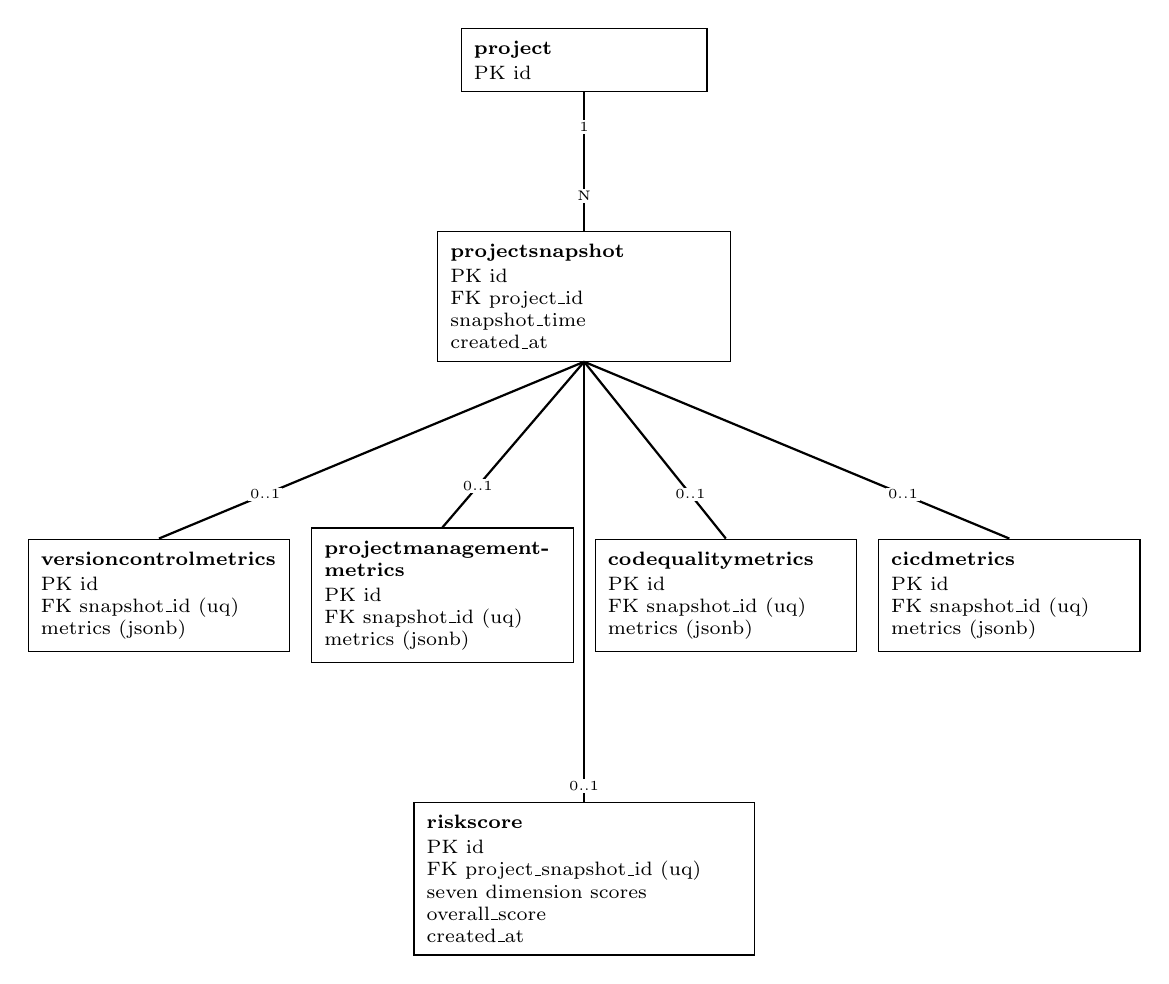
\begin{tikzpicture}[
  font=\scriptsize,
  ent/.style={draw, align=left, inner sep=1.6mm},
  rel/.style={thick},
  card/.style={font=\tiny, fill=white, inner sep=0.8pt}
]
\node[ent, text width=28mm] (proj) at (0mm,0mm)
  {\textbf{project}\\[1pt] PK id};

\node[ent, text width=34mm] (snap) at (0mm,-30mm)
  {\textbf{projectsnapshot}\\[1pt] PK id\\ FK project\_id\\ snapshot\_time\\
created\_at};

\node[ent, text width=30mm] (vcm) at (-54mm,-68mm)
  {\textbf{versioncontrolmetrics}\\[1pt] PK id\\ FK snapshot\_id (uq)\\ metrics
(jsonb)};
\node[ent, text width=30mm] (pmm) at (-18mm,-68mm)
  {\textbf{projectmanagement\-metrics}\\[1pt] PK id\\ FK snapshot\_id (uq)\\ metrics
(jsonb)};
\node[ent, text width=30mm] (cqm) at (18mm,-68mm)
  {\textbf{codequalitymetrics}\\[1pt] PK id\\ FK snapshot\_id (uq)\\ metrics
(jsonb)};
\node[ent, text width=30mm] (cicd) at (54mm,-68mm)
  {\textbf{cicdmetrics}\\[1pt] PK id\\ FK snapshot\_id (uq)\\ metrics (jsonb)};

\node[ent, text width=40mm] (risk) at (0mm,-104mm)
  {\textbf{riskscore}\\[1pt] PK id\\ FK project\_snapshot\_id (uq)\\
   seven dimension scores\\ overall\_score\\ created\_at};

\draw[rel] (proj.south) -- node[card, near start] {1} node[card, near end] {N}
(snap.north);
\draw[rel] (snap.south) -- node[card, near end] {0..1} (vcm.north);
\draw[rel] (snap.south) -- node[card, near end] {0..1} (pmm.north);
\draw[rel] (snap.south) -- node[card, near end] {0..1} (cqm.north);
\draw[rel] (snap.south) -- node[card, near end] {0..1} (cicd.north);
\draw[rel] (snap.south) -- (0mm,-86mm) -- node[card, near end] {0..1} (risk.north);
\end{tikzpicture}
\caption{Metric capture and scoring. A snapshot is an immutable record of one
synchronisation; the unique constraint on each child table admits at most one row
per snapshot per tool, and a snapshot for which a tool was unconfigured or failed
simply has no corresponding row.}
\label{fig:erd-metrics}
\end{figure}

\begin{figure}[htbp]
\centering
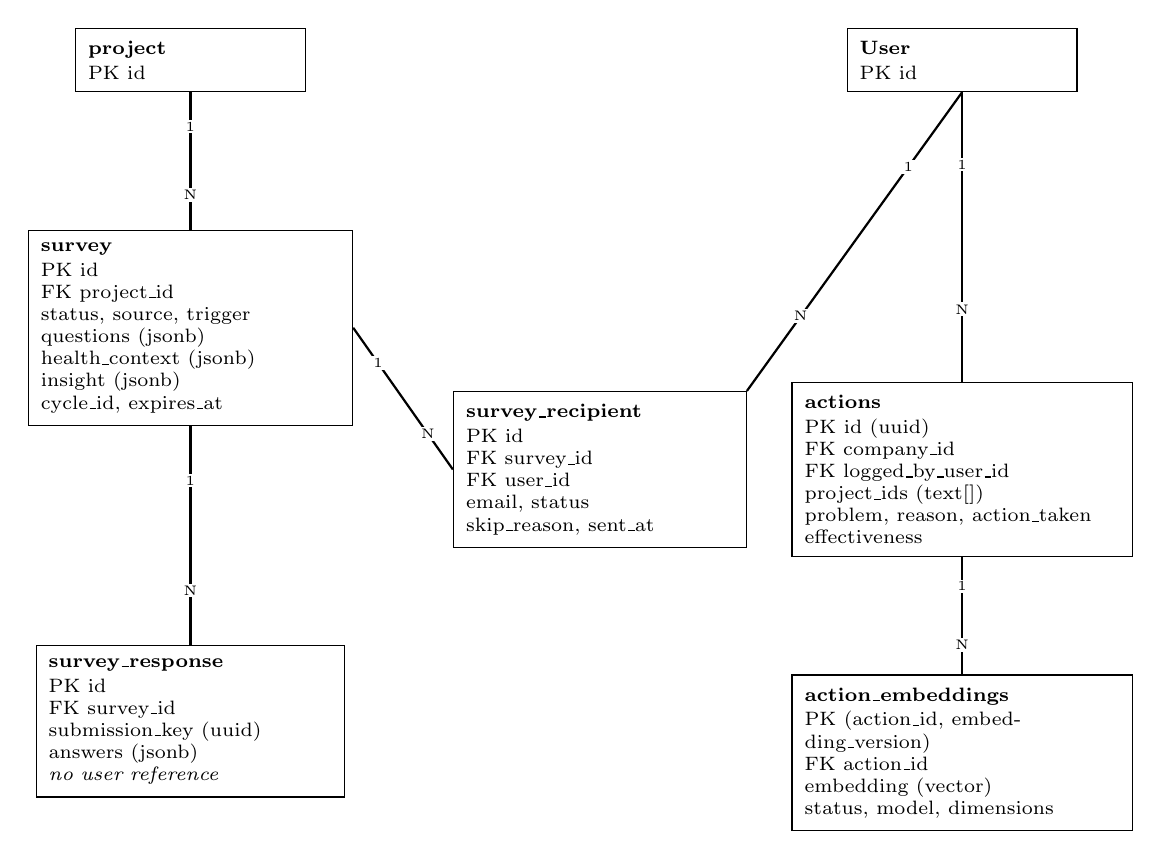
\begin{tikzpicture}[
  font=\scriptsize,
  ent/.style={draw, align=left, inner sep=1.6mm},
  rel/.style={thick},
  weak/.style={thick, dashed},
  card/.style={font=\tiny, fill=white, inner sep=0.8pt}
]
\node[ent, text width=26mm] (proj) at (-52mm,0mm)
  {\textbf{project}\\[1pt] PK id};
\node[ent, text width=26mm] (usr) at (46mm,0mm)
  {\textbf{User}\\[1pt] PK id};

\node[ent, text width=38mm] (srv) at (-52mm,-34mm)
  {\textbf{survey}\\[1pt] PK id\\ FK project\_id\\ status, source, trigger\\
   questions (jsonb)\\ health\_context (jsonb)\\ insight (jsonb)\\
   cycle\_id, expires\_at};

\node[ent, text width=36mm] (resp) at (-52mm,-84mm)
  {\textbf{survey\_response}\\[1pt] PK id\\ FK survey\_id\\ submission\_key (uuid)\\
   answers (jsonb)\\ \emph{no user reference}};

\node[ent, text width=34mm] (rcp) at (0mm,-52mm)
  {\textbf{survey\_recipient}\\[1pt] PK id\\ FK survey\_id\\ FK user\_id\\
   email, status\\ skip\_reason, sent\_at};

\node[ent, text width=40mm] (act) at (46mm,-52mm)
  {\textbf{actions}\\[1pt] PK id (uuid)\\ FK company\_id\\ FK logged\_by\_user\_id\\
   project\_ids (text[])\\ problem, reason, action\_taken\\ effectiveness};

\node[ent, text width=40mm] (emb) at (46mm,-88mm)
  {\textbf{action\_embeddings}\\[1pt] PK (action\_id, embedding\_version)\\
   FK action\_id\\ embedding (vector)\\ status, model, dimensions};

\draw[rel] (proj.south) -- node[card, near start] {1} node[card, near end] {N}
(srv.north);
\draw[rel] (srv.south) -- node[card, near start] {1} node[card, near end] {N}
(resp.north);
\draw[rel] (srv.east) -- node[card, near start] {1} node[card, near end] {N}
(rcp.west);
\draw[rel] (usr.south) -- node[card, near start] {1} node[card, near end] {N}
(rcp.north east);
\draw[rel] (usr.south) -- node[card, near start] {1} node[card, near end] {N}
(act.north);
\draw[rel] (act.south) -- node[card, near start] {1} node[card, near end] {N}
(emb.north);
% \draw[weak] (proj.north) -- (-52mm,14mm) -- (46mm,14mm)
%   node[card, midway, above] {referenced by value, not by key} (act.north west);
\end{tikzpicture}
\caption{Surveys and management actions. Two relationships are deliberately
absent as foreign keys: a survey response holds no reference to the respondent,
and an action names its projects in a text array rather than through a join
table.}
\label{fig:erd-engagement}
\end{figure}

\paragraph{Immutable snapshots.}
The central structural decision is that a synchronisation produces an
append-only record. A \texttt{projectsnapshot} row is created per run, each
tool's output is attached to it, and the computed scores are attached to the same
row; nothing is ever updated in place. Trend data is therefore a by-product of
the storage model rather than a separate concern, and any historical score
remains attributable to the exact inputs that produced it which is what makes
the on-demand score breakdown of FR-26 possible.

\paragraph{Semi-structured metric storage.}
Each of the four metric tables holds a single \texttt{jsonb} column rather than a
column per metric. This was a revision made during implementation, discussed in
\Cref{subsec:design-refinement}, and it reflects the reality that each connector
returns a deeply nested, provider-specific structure which evolves as a
connector's coverage improves. Relational columns would have required a schema
migration for every metric added, whereas the scoring layer reads the fields it
needs by name and tolerates their absence by design (FR-22).

\paragraph{Anonymity enforced structurally.}
\texttt{survey\_response} carries a randomly generated \texttt{submission\_key}
and no reference to any user. The system records separately, in
\texttt{survey\_recipient}, who was invited to a survey, but there is no
column anywhere linking an invitation to a response. The anonymity guarantee of
NFR-07 is therefore a property of the schema, not of application logic. No query
can reconstruct the association, and no future change to the service layer can
accidentally expose it.

\paragraph{Actions referenced by value.}
An action names the projects it concerns in a \texttt{text[]} column rather than
through a join table. This is a deliberate denormalisation. An action is a
managerial narrative that may span several projects, is queried almost
exclusively by containment, and carries no per-project attributes that a join
table would hold. The cost is the loss of referential integrity to
\texttt{project}, which the application compensates for by validating project
membership at write time.

\paragraph{Versioned embeddings.}
\texttt{action\_embeddings} is keyed on the pair
\texttt{(action\_id, embedding\_version)} rather than on the action alone, so that
vectors produced by different models or dimensionalities coexist. This permits an
embedding model to be replaced by generating a new version alongside the old one
and switching over once backfill completes, rather than by a destructive
migration. This capability was exercised when the embedding provider was
changed during development.


\subsection{Synchronisation Sequence}
\label{subsec:sync-sequence}

\Cref{fig:sync-sequence} traces one user-initiated synchronisation from the
button press to the updated dashboard. The client opens its progress stream before submitting
the synchronisation request, so that events emitted by a fast connector cannot
occur in the gap between the request returning and the stream being established.
No progress event travels directly from the worker to the browser. The
worker performs the work but holds no connection to the client, so every event is
published to Redis, relayed by the API process, and forwarded over Server-Sent
Events.

\begin{figure}[htbp]
\centering
\begin{tikzpicture}[
  font=\scriptsize,
  head/.style={draw, rounded corners=1pt, align=center, text width=19mm,
               inner sep=1.2mm, font=\scriptsize},
  life/.style={dashed, gray},
  msg/.style={-{Stealth[length=1.6mm]}, thin},
  ret/.style={-{Stealth[length=1.6mm]}, thin, dashed},
  lbl/.style={font=\tiny, above, fill=white, inner sep=0.6pt},
  frame/.style={draw, thin, gray},
  ftag/.style={font=\tiny\itshape, anchor=north west, inner sep=1pt}
]

%% ---------- participants ----------
\node[head] (client) at (0mm,0mm)   {Web client};
\node[head] (api)    at (25mm,0mm)  {API process};
\node[head] (redis)  at (50mm,0mm)  {Redis};
\node[head] (worker) at (75mm,0mm)  {Worker process};
\node[head] (ext)    at (100mm,0mm) {External tool APIs};
\node[head] (db)     at (125mm,0mm) {PostgreSQL};

\foreach \x in {0,25,50,75,100,125}
  \draw[life] (\x mm,-7mm) -- (\x mm,-176mm);

%% ---------- setup ----------
\draw[msg] (0mm,-16mm)  -- node[lbl] {GET /projects/:id} (25mm,-16mm);
\draw[msg] (0mm,-23mm)  -- node[lbl] {GET /progress/:sid (SSE)} (25mm,-23mm);
\draw[msg] (25mm,-30mm) -- node[lbl] {subscribe to channel} (50mm,-30mm);
\draw[msg] (0mm,-37mm)  -- node[lbl] {POST /sync} (25mm,-37mm);
\draw[msg] (25mm,-44mm) -- node[lbl] {load integrations, decrypt} (125mm,-44mm);
\draw[msg] (25mm,-51mm) -- node[lbl] {enqueue job} (50mm,-51mm);
\draw[ret] (25mm,-58mm) -- node[lbl] {202 Accepted} (0mm,-58mm);
\draw[msg] (50mm,-65mm) -- node[lbl] {dequeue} (75mm,-65mm);

%% ---------- frame A: per tool, concurrent ----------
\draw[frame] (-13mm,-71mm) rectangle (113mm,-102mm);
\node[ftag] at (-13mm,-71mm) {~loop [per configured tool, concurrent]};
\draw[msg] (75mm,-79mm) -- node[lbl] {publish ``syncing''} (50mm,-79mm);
\draw[ret] (50mm,-86mm) -- node[lbl] {event} (25mm,-86mm);
\draw[ret] (25mm,-93mm) -- node[lbl] {SSE progress update} (0mm,-93mm);
\draw[msg] (75mm,-100mm) -- node[lbl] {fetch metrics} (100mm,-100mm);

%% ---------- snapshot ----------
\draw[msg] (75mm,-109mm) -- node[lbl] {create snapshot} (125mm,-109mm);

%% ---------- frame B: per successful tool ----------
\draw[frame] (-13mm,-115mm) rectangle (137mm,-139mm);
\node[ftag] at (-13mm,-115mm) {~loop [per successful tool, sequential]};
\draw[msg] (75mm,-123mm) -- node[lbl] {persist normalised metrics} (125mm,-123mm);
\draw[msg] (75mm,-130mm) -- node[lbl] {publish ``completed''} (50mm,-130mm);
\draw[ret] (50mm,-137mm) -- node[lbl] {relayed to client} (0mm,-137mm);

%% ---------- scoring and completion ----------
\draw[msg] (75mm,-147mm) -- node[lbl] {publish ``calculating risk''} (50mm,-147mm);
\draw[msg] (75mm,-154mm) -- node[lbl] {read metrics, compute, store scores}
(125mm,-154mm);
\draw[msg] (75mm,-161mm) -- node[lbl] {publish completion (retained 1\,h)}
(50mm,-161mm);
\draw[ret] (50mm,-168mm) -- node[lbl] {completion event} (25mm,-168mm);
\draw[ret] (25mm,-175mm) -- node[lbl] {SSE completion; stream closes} (0mm,-175mm);
\end{tikzpicture}
\caption{Synchronisation sequence. Solid arrows are requests and commands; dashed
arrows are responses and relayed events. Progress reaches the browser only by
being published to Redis and forwarded by the API process, because the worker
holds no client connection.}
\label{fig:sync-sequence}
\end{figure}

\paragraph{Ordering of fetch and persistence.}
The two loop fragments differ deliberately. Fetching is performed concurrently
across the configured tools, bounded by a concurrency limit, because the four
external APIs are independent and the elapsed time of a synchronisation is
dominated by network latency. Persistence is performed sequentially afterwards,
because every tool's output must attach to the same snapshot row. The snapshot is
created once, after at least one fetch has succeeded, and each tool's metrics are
then written against it. Creating the snapshot before the persistence loop rather
than lazily within it ensures that a failure part-way through cannot leave one
synchronisation's data split across two snapshot rows.

\paragraph{Partial completion.}
A tool that fails at either stage emits a failure event and is recorded in the
job's failed list, but does not abort the run (FR-19, NFR-10). The completion
event therefore carries three possible outcomes which are success, partial, or failed, 
derived from which tools succeeded, and additionally downgraded from success to partial 
if scoring itself failed, so that a run which collected data but
produced no usable score is not reported to the user as wholly successful.

\paragraph{Reconnection.}
The completion event is not only published but also retained in Redis for one
hour. When a client opens a progress stream, the API first checks for a retained
completion for that session and, if one exists, delivers it immediately and
closes the stream. This is what allows a user to reload the page or navigate away
during a long synchronisation and still receive its outcome on return (FR-17),
rather than subscribing to a channel on which nothing further will ever be
published.


\subsection{Application Programming Interface}
\label{subsec:api-surface}

The server exposes 54 HTTP endpoints beneath the version prefix
\texttt{/api/v1}, which is omitted from the paths listed in
\Cref{tab:api-surface}. The interface follows REST conventions in resource
naming and method semantics, with one deliberate exception: the progress endpoint
is a Server-Sent Events stream rather than a request-response resource, because
the client must receive an unbounded series of events for a single logical
operation.

\paragraph{Conventions.}
Authentication is carried by an \texttt{httpOnly} session cookie rather than a
bearer token. This suits a single-page client served from the same origin as the
API. The browser automatically attaches the cookie, including on the
\texttt{EventSource} connection used for progress streaming, which cannot carry
custom headers. Errors return a uniform \texttt{\{ message \}} body with a status
code distinguishing the cause. The status codes are 400 for malformed input, 401 for an absent or
expired session, 403 for an authenticated caller lacking rights to the resource,
404 for a resource outside the caller's company (so that cross-tenant probing
cannot distinguish "forbidden" from "nonexistent"), 409 for a conflicting state,
and 503 where an optional external capability is unavailable. Successful
mutations return 200 or 201, except synchronisation, which returns 202 to signal
that work has been accepted but not performed.

Within each router, literal path segments are registered before parameterised
ones --- \texttt{/projects/health} before \texttt{/projects/:id},
\texttt{/actions/search} before \texttt{/actions/:id} --- so that a literal
segment is not captured as an identifier by a more general route declared
earlier.

\begin{longtable}{
  >{\raggedright\arraybackslash}p{0.09\textwidth}
  >{\ttfamily\scriptsize\raggedright\arraybackslash}p{0.29\textwidth}
  >{\raggedright\arraybackslash}p{0.30\textwidth}
  >{\raggedright\arraybackslash}p{0.18\textwidth}
}
\caption{Endpoint inventory, excluding the \texttt{/api/v1} prefix}
\label{tab:api-surface}\\
\toprule
\textbf{Method} & \textbf{\normalsize\rmfamily Path} & \textbf{Purpose} &
\textbf{Auth required} \\
\midrule
\endfirsthead
\toprule
\textbf{Method} & \textbf{\normalsize\rmfamily Path} & \textbf{Purpose} &
\textbf{Auth required} \\
\midrule
\endhead
\bottomrule
\endlastfoot
\multicolumn{4}{l}{\textit{Service health}} \\
GET & /health & Service and dependency status & None \\
\addlinespace
\multicolumn{4}{l}{\textit{Authentication and account lifecycle}} \\
POST & /auth/send-verification-code & Email a signup verification code & None \\
POST & /auth/verify-email-code & Confirm a verification code & None \\
POST & /auth/register & Create a company and administrator, or join by invitation &
None \\
POST & /auth/login & Authenticate and open a session & None \\
POST & /auth/logout & Revoke the current session & None \\
GET & /auth/me & Resolve the authenticated user & Session \\
POST & /auth/forgot-password & Email a password reset link & None \\
POST & /auth/reset-password & Consume a reset token and revoke all sessions & None \\
GET & /auth/invite/:token & Inspect an invitation without consuming it & None \\
POST & /auth/accept-invite & Join a project as an existing user & Session \\
\addlinespace
\multicolumn{4}{l}{\textit{Workspaces and repository import}} \\
GET & /workspaces & List the company's workspaces & Session \\
POST & /workspaces & Create a workspace and import repositories & Session,
administrator \\
POST & /workspaces/preview-repos & List repositories reachable with a token, storing
nothing & Session, administrator \\
GET & /workspaces/:workspaceId/repos & List repositories, flagging those already
imported & Session, administrator \\
POST & /workspaces/:workspaceId/projects & Import further repositories as projects &
Session, administrator \\
\addlinespace
\multicolumn{4}{l}{\textit{Projects, health and configuration}} \\
GET & /projects & List accessible projects with latest scores & Session \\
GET & /projects/health & Dashboard feed: every accessible project with score history
& Session \\
GET & /projects/:id & Project detail, integrations and members & Session \\
GET & /projects/:projectId/health & Health history for one project & Session \\
GET & /projects/:projectId/snapshots /:snapshotId/score-breakdown /:scoreType &
Per-metric breakdown of one score & Session \\
PATCH & /projects/:projectId/integrations & Create or update a tool integration &
Session, administrator \\
PATCH & /projects/:projectId/tracked & Toggle portfolio tracking & Session,
administrator \\
POST & /projects/:projectId/invites & Invite a member by email & Session,
administrator \\
DELETE & /projects/:projectId/members /:userId & Remove a member & Session,
administrator \\
GET & /projects/:projectId/integrations /:toolName/token & Reveal the effective
credential & Session, administrator \\
\addlinespace
\multicolumn{4}{l}{\textit{Synchronisation}} \\
POST & /sync & Enqueue a synchronisation job & Session, project access \\
GET & /sync/:jobId & Inspect job state & Session \\
GET & /progress/:sessionId & Server-Sent Events progress stream & Session \\
\addlinespace
\multicolumn{4}{l}{\textit{Surveys, administrative}} \\
GET & /surveys & List surveys across projects & Requester-role header \\
GET & /surveys/:surveyId & Survey detail, responses and analysis & Requester-role
header \\
PATCH & /surveys/:surveyId/questions & Edit questions before dispatch &
Requester-role header \\
PATCH & /surveys/:surveyId/complete & Close and queue analysis & Requester-role
header \\
POST & /surveys/:surveyId/close & Close an active survey & Requester-role header \\
POST & /surveys/:surveyId/remind & Rebroadcast the link & Requester-role header \\
PATCH & /surveys/:surveyId/lifecycle & Pause, resume, retry or cancel &
Requester-role header \\
\addlinespace
\multicolumn{4}{l}{\textit{Surveys, project-scoped}} \\
POST & /projects/:projectId/surveys /generate-questions & Generate and score candidate
questions & Requester-role header \\
POST & /projects/:projectId/surveys /send-now & Create and dispatch immediately &
Requester-role header \\
POST & /projects/:projectId/surveys & Create and dispatch with supplied questions &
Requester-role header \\
GET & /projects/:projectId/surveys & List a project's surveys & Requester-role header
\\
GET & /projects/:projectId/surveys/quota & Remaining manual dispatches this month &
Requester-role header \\
GET & /projects/:projectId/surveys /schedule & Current month's scheduled pulse &
Requester-role header \\
GET & /projects/:projectId/pending-survey & Whether the project is flagged as due &
Requester-role header \\
\addlinespace
\multicolumn{4}{l}{\textit{Surveys, public respondent interface}} \\
GET & /public/surveys/:token & Retrieve the form behind an anonymous link & Token,
rate-limited \\
POST & /public/surveys/:token/responses & Submit an anonymous response & Token,
rate-limited \\
\addlinespace
\multicolumn{4}{l}{\textit{Management actions}} \\
POST & /actions & Record an action & Session \\
GET & /actions & List actions, scoped by role & Session \\
GET & /actions/search & Keyword or semantic search & Session \\
GET & /actions/effectiveness-review & Actions awaiting the author's review & Session
\\
GET & /actions/:id & Retrieve one action & Session \\
PUT & /actions/:id & Amend an action & Session \\
DELETE & /actions/:id & Delete an action & Session \\
PUT & /actions/:id/effectiveness & Rate effectiveness & Session, author only \\
PUT & /actions/:id/review-schedule & Defer the review & Session, author only \\
\end{longtable}

\paragraph{Tenancy scoping.}
Every endpoint marked \emph{Session} resolves the caller's company from the
session and restricts its query to that company. Project-scoped endpoints apply a
second check: an administrator may reach any project within their company, while
a member must additionally hold a membership record for the specific project. The
score-breakdown endpoint applies a third, because snapshot identifiers are
sequential across all projects and would otherwise be enumerable. It confirms
that the named snapshot belongs to the named project before serving it.

\paragraph{The public respondent interface.}
Two endpoints are reachable without a session, by design. A survey respondent is
not a user of the system and holds no account. Authorisation is carried instead
by the encrypted link token, which names the survey, its distribution cycle and
its deadline, and is sealed such that altering any of those fails decoding.
Because these endpoints are the system's only unauthenticated write surface, they
carry request rate limits, sixty form retrievals and ten submissions per
fifteen-minute window as defence in depth behind the token's own entropy.



\subsection{Design Calculations}
\label{subsec:design-calculations}

Two constraints established in \Cref{subsec:constraints} required
quantitative verification rather than assertion, the system had to operate
entirely within free service tiers (C-03), and it had to respect the rate limits
published by external providers (NFR-16). The estimates below were derived from
the connector metric schemas and the configured synchronisation cadence, and
determine whether the chosen parameters actually satisfy those constraints.

\paragraph{Storage per snapshot.}
Each synchronisation writes one \texttt{projectsnapshot} row, up to four metric
rows and one \texttt{riskscore} row. The metric payloads dominate. Their size was
estimated by counting the leaf fields of each connector's response type and
allowing approximately 38 bytes per field for the key string, value and
\texttt{jsonb} entry overhead, plus the contribution of the variable-length
arrays.

\begin{longtable}{
  >{\raggedright\arraybackslash}p{0.30\textwidth}
  >{\raggedright\arraybackslash}p{0.38\textwidth}
  >{\raggedright\arraybackslash}p{0.16\textwidth}
}
\caption{Estimated storage per snapshot}
\label{tab:storage-per-snapshot}\\
\toprule
\textbf{Component} & \textbf{Basis} & \textbf{Estimate} \\
\midrule
\endfirsthead
\toprule
\textbf{Component} & \textbf{Basis} & \textbf{Estimate} \\
\midrule
\endhead
\bottomrule
\endlastfoot
versioncontrolmetrics & 31 scalar fields, plus one entry per top-level directory
touched (assumed 15) & 2.3 kB \\
projectmanagementmetrics & 25 scalar fields, plus a sprint trend capped at 10 entries
& 1.5 kB \\
codequalitymetrics & 21 scalar fields, plus hotspot files capped at 5 entries & 1.2
kB \\
cicdmetrics & 10 scalar fields & 0.4 kB \\
projectsnapshot, riskscore and row overhead & Fixed-width columns & 0.3 kB \\
\midrule
\textbf{Total per snapshot} & & \textbf{$\approx$ 5.7 kB} \\
\end{longtable}

\paragraph{Storage growth.}
With the default schedule of one synchronisation per project per day, a project
accumulates 365 snapshots per year, or approximately 2.1\,MB. Allowing roughly
thirty per cent for indexes gives 2.7\,MB per project-year for scheduled
synchronisation alone. Manual synchronisation adds to this in direct proportion.
A team synchronising once more per working day approximately doubles the figure,
to about 5.4\,MB per project-year.

\begin{longtable}{
  >{\raggedright\arraybackslash}p{0.26\textwidth}
  >{\raggedright\arraybackslash}p{0.20\textwidth}
  >{\raggedright\arraybackslash}p{0.20\textwidth}
  >{\raggedright\arraybackslash}p{0.18\textwidth}
}
\caption{Projected database growth for a 25-project portfolio}
\label{tab:storage-growth}\\
\toprule
\textbf{Usage} & \textbf{Per project-year} & \textbf{25 projects, 3 years} &
\textbf{Free tier reached} \\
\midrule
\endfirsthead
\toprule
\textbf{Usage} & \textbf{Per project-year} & \textbf{25 projects, 3 years} &
\textbf{Free tier reached} \\
\midrule
\endhead
\bottomrule
\endlastfoot
Scheduled only & 2.7 MB & 203 MB & $\approx$ 7 years \\
Scheduled plus daily manual & 5.4 MB & 405 MB & $\approx$ 3.7 years \\
\end{longtable}

This is the least comfortable of the estimates. The managed database's free tier
provides 500\,MB, so a portfolio of twenty-five projects remains within it for
somewhere between four and seven years depending on how often users synchronise
manually --- adequate for the project's horizon, but not indefinitely. The
append-only snapshot model is what consumes the space, and it is also what makes
the remedy straightforward. Since each snapshot is self-contained, snapshots
older than a retention horizon can be deleted, or thinned to weekly resolution,
without affecting any other record. No such pruning is implemented, and it is
recorded as future work.

\paragraph{External request budget.}
The version-control connector dominates the request count, because it retrieves
the file list of every commit in a thirty-day window individually. For a
repository receiving approximately 200 commits per month the budget is as
follows.

\begin{longtable}{
  >{\raggedright\arraybackslash}p{0.40\textwidth}
  >{\raggedright\arraybackslash}p{0.44\textwidth}
}
\caption{Estimated version-control API requests per synchronisation}
\label{tab:api-budget}\\
\toprule
\textbf{Operation} & \textbf{Requests} \\
\midrule
\endfirsthead
\toprule
\textbf{Operation} & \textbf{Requests} \\
\midrule
\endhead
\bottomrule
\endlastfoot
Per-commit file detail (200 commits, concurrency 4) & $\approx$ 200 \\
Commit and closed-issue listing (paginated, 100 per page) & 3--4 \\
Pull requests with reviews, issues, branches (GraphQL) & 5--15 queries \\
Default branch, dependency alerts, secret-scanning alerts & 3--4 \\
\midrule
\textbf{Total per synchronisation} & \textbf{$\approx$ 210--260} \\
\end{longtable}

An authenticated personal access token permits 5{,}000 REST requests per hour,
which bounds the system at roughly nineteen to twenty-four synchronisations per
hour per credential. The scheduled fan-out spaces projects sharing a credential
ten minutes apart, producing at most six synchronisations per hour, or
approximately 1{,}500 requests which is around thirty per cent of the available
budget. The chosen spacing therefore satisfies NFR-16 with a headroom factor of
roughly three.

This holds up to eighteen projects per credential. Beyond that, the
180-minute cap on total spread causes further projects to be scheduled at the
same moment rather than spaced further apart, and the headroom narrows. A
workspace substantially larger than eighteen repositories would require the
spacing or cap to be reconsidered, which is why both are configurable rather than
fixed.

\paragraph{Worker throughput.}
Synchronisation duration is dominated by the same per-commit requests, issued at
a concurrency of four; together with the other three connectors, which run
concurrently with the version-control connector, a synchronisation is estimated
at one to three minutes for a repository of the size assumed above. The worker
processes two synchronisation jobs in parallel, so a twenty-five-project
scheduled run occupies approximately twenty-five to forty minutes of wall-clock
time. This fits comfortably within the 180-minute window over which the run is
spread, confirming that the queue is not the limiting factor but the deliberate
spacing is.

\paragraph{Cache and vector storage.}
The in-memory store holds three kinds of data, all small. Sessions are
approximately 200 bytes each with a one-day expiry. Queued jobs carry the
project's resolved integration credentials and are approximately 2--4\,kB each;
scheduled jobs retain their completed record for twenty-five hours so that their
deterministic identifiers stay reserved, giving roughly 100\,kB for a
twenty-five-project run. Retained completion events expire after one hour. The
total working set is well under one megabyte, against a free-tier allowance
measured in hundreds. Action embeddings occupy 768 four-byte components plus row
overhead, approximately 3.3\,kB per action, so even a corpus of a thousand
actions adds only some 3\,MB.

\paragraph{Conclusion.}
The calculations confirm that the design satisfies C-03 and NFR-16 with the
chosen parameters, and identify where each constraint would eventually bind: the
database free tier at roughly four to seven years of accumulated history for a
mid-sized portfolio, and the version-control rate limit at approximately eighteen
projects sharing a single credential. Both limits are addressed by configuration
rather than redesign which is a retention policy in the first case, and the already
configurable spacing and spread parameters in the second.




\subsection{Verification of the Design}
\label{subsec:design-verification}

Verification was applied at four levels, chosen so that each class of design risk
is checked by the cheapest mechanism capable of detecting it: static analysis for
type and contract errors, unit tests for the scoring model's arithmetic, live-API
scripts for connector behaviour against real providers, and end-to-end scripts
for the assembled pipeline.

\paragraph{Static verification.}
The entire codebase is written in a statically typed language with strict
compiler settings, and the connector and scoring layers are typed generically.
Each scoring strategy declares the metric object it consumes, so supplying a
strategy with the wrong metric type is a compile-time error rather than a runtime
one. Type checking and static analysis run on every change through continuous
integration (\Cref{sec:implementation}), which means a change that breaks a
contract between modules cannot reach the main branch.

\paragraph{Unit verification of the scoring model.}
The scoring model received the heaviest test coverage, because it is the
component whose failures are least visible. A connector that breaks produces an
obvious error, whereas a scoring defect produces a plausible but wrong number. Of
the 131 automated test cases, 83 target the risk engine.

\begin{longtable}{
  >{\raggedright\arraybackslash}p{0.34\textwidth}
  >{\raggedright\arraybackslash}p{0.12\textwidth}
  >{\raggedright\arraybackslash}p{0.38\textwidth}
}
\caption{Automated test coverage by area}
\label{tab:test-coverage}\\
\toprule
\textbf{Area} & \textbf{Cases} & \textbf{What is verified} \\
\midrule
\endfirsthead
\toprule
\textbf{Area} & \textbf{Cases} & \textbf{What is verified} \\
\midrule
\endhead
\bottomrule
\endlastfoot
Shared scoring functions & 26 & Normalisation at boundary values, weight
renormalisation when signals are absent, clamping of out-of-range inputs \\
Seven scoring strategies & 57 & Each dimension's best case scores 100 and worst case
0; weights match the documented rules; missing metrics are excluded rather than
treated as zero \\
Credential encryption & 4 & Round-trip correctness, distinct ciphertexts for
identical input, rejection of tampered ciphertext \\
Survey link tokens & 5 & Round-trip correctness, expiry detection, rejection of
tampered or malformed tokens \\
Survey question generation & 6 & Deduplication, quality gating, category diversity in
selection \\
Survey response validation & 6 & Answer-type conformance, rejection of answers
outside the survey \\
Scheduled synchronisation & 6 & Credential grouping, spacing and spread clamping,
deterministic job identifiers, continuation after one project fails \\
Timestamp handling & 7 & Correct interpretation of zone-naive and zone-aware values
\\
Concurrency helper and connector concurrency & 4 & Bounded parallelism, preservation
of result order \\
Semantic search, embeddings, reranking & 3 suites & Provider adapters and fallback
behaviour \\
\end{longtable}

The scoring tests are written against the published rules rather than against the
implementation, which is what allowed the restructuring from six categories to
seven to proceed with confidence. The tests encoded what each dimension was specified to produce, so a change that altered behaviour unintentionally
failed visibly.

\paragraph{Verification of connectors against live providers.}
Connector behaviour cannot be verified by unit tests alone, because the risk
being checked is precisely whether the provider's API behaves as the
implementation assumes. A separate script exists for each connector
(\texttt{test-github-metrics}, \texttt{test-jira},
\texttt{test-sonarqube-metrics}, \texttt{test-github-actions-metrics}), each of
which runs that connector against a real project and prints the complete
normalised metric object. These were used throughout development to confirm that
every field the scoring model expects is actually populated by real data, and to
identify the fields that are not. The unavailability of security alert counts
where scanning is disabled, and of coverage where no report is published, both
recorded as constraint C-05, were discovered this way rather than anticipated.

\paragraph{End-to-end verification of the pipeline.}
Two scripts verify the assembled system. \texttt{test-risk-scores} runs all four
connectors against a single real project and produces all seven scores,
exercising the complete path from provider APIs through normalisation and
persistence to the scoring engine which is the same path
\Cref{fig:connector-scoring} describes. A second script performs a smoke test of
the deployed stack. It confirms the API's health endpoint reports its
dependencies as reachable, confirms database connectivity, enqueues a
synchronisation job, and polls its status, thereby exercising the queue and
worker boundary that unit tests cannot reach.

\paragraph{Requirement traceability.}
\Cref{tab:verification-traceability} maps the requirements whose satisfaction
depends on design decisions rather than on straightforward implementation to the
verification that covers each.

\begin{longtable}{
  >{\raggedright\arraybackslash}p{0.14\textwidth}
  >{\raggedright\arraybackslash}p{0.36\textwidth}
  >{\raggedright\arraybackslash}p{0.34\textwidth}
}
\caption{Verification of design-critical requirements}
\label{tab:verification-traceability}\\
\toprule
\textbf{Requirement} & \textbf{Property to be verified} & \textbf{Verified by} \\
\midrule
\endfirsthead
\toprule
\textbf{Requirement} & \textbf{Property to be verified} & \textbf{Verified by} \\
\midrule
\endhead
\bottomrule
\endlastfoot
FR-22 & Scores computed from partial data, absent weights redistributed & Unit tests
on the shared weighting function and on each strategy \\
FR-19, NFR-10 & One tool failing does not abort a synchronisation & Scheduled-sync
processor tests; observed during live connector runs \\
NFR-12 & Repeated schedule triggers do not duplicate work & Scheduled-sync processor
tests on deterministic job identifiers \\
NFR-16 & External rate limits respected & Design calculation
(\Cref{subsec:design-calculations}); concurrency tests \\
NFR-01 & Credentials encrypted at rest & Encryption round-trip and tamper-rejection
tests \\
NFR-06 & Survey links tamper-evident & Token tamper-rejection tests \\
NFR-15 & Bounded concurrency on external calls & Concurrency helper tests \\
O-07, NFR-21 & New providers addable without changing scoring & Demonstrated
structurally by the placeholder connectors \\
\end{longtable}

\paragraph{Limitations of the verification performed.}
Three limitations should be stated. First, no automated integration tests execute
against a live database or queue; the boundary between the application and its
infrastructure is covered only by the manual test script. Second, the
connector verification scripts are observational rather than assertive. They
print their output for inspection rather than asserting expected values, which is
appropriate for data whose correct value changes with the repository but means
they cannot run unattended in continuous integration. Third, the calibration
constants in the scoring model are verified for internal consistency but not for
external validity. The tests confirm that a metric at its defined best scores
100, not that the threshold defining "best" is the right one. That remains open
work requiring real project outcomes to calibrate against.




\subsection{Design Refinements During Implementation}
\label{subsec:design-refinement}

The design described in this chapter is not the design the project began with.
Several structures were revised once implementation exposed problems that were
not visible on paper, and the schema migration history which includes seventeen migrations,
each recording its own rationale is the record of that revision.
\Cref{tab:refinements} summarises the changes that altered the design rather than
merely extending it.

\begin{longtable}{
  >{\raggedright\arraybackslash}p{0.26\textwidth}
  >{\raggedright\arraybackslash}p{0.28\textwidth}
  >{\raggedright\arraybackslash}p{0.30\textwidth}
}
\caption{Design refinements made during implementation}
\label{tab:refinements}\\
\toprule
\textbf{Change} & \textbf{Problem it addressed} & \textbf{Effect on the design} \\
\midrule
\endfirsthead
\toprule
\textbf{Change} & \textbf{Problem it addressed} & \textbf{Effect on the design} \\
\midrule
\endhead
\bottomrule
\endlastfoot
Per-tool credential columns on \texttt{project} replaced by a generic integration
table with a \texttt{jsonb} configuration & Twelve tool-specific columns had
accumulated; each new tool required further columns and a migration & Adding a tool
became a data change rather than a schema change \\
\addlinespace
Metric tables collapsed from one column per metric to a single \texttt{jsonb} column
& Every metric a connector gained required a migration, and the connector outputs are
nested rather than flat & Connector coverage could expand freely; the scoring layer
reads fields by name and tolerates absence \\
\addlinespace
Access tokens moved from individual projects onto the owning workspace & The same
credential was duplicated across every project imported from one organisation,
multiplying the cost of rotation & One credential per workspace, resolved at
synchronisation time \\
\addlinespace
Scoring model restructured from six risk categories to seven health dimensions & The
original categories conflated concerns the available metrics could distinguish, and
were oriented so that a lower score was better & Scores became uniformly
higher-is-better; columns were dropped rather than renamed \\
\addlinespace
Overall score changed from computed-on-read to persisted at synchronisation & The
aggregate was recomputed on every dashboard request and could not be indexed or
compared historically & One stored value per snapshot, computed by the same
null-aware mechanism as its components \\
\addlinespace
Timestamp columns converted from zone-naive to zone-aware & Values written as UTC
lost their offset on storage and were reinterpreted as local time by every client &
Chart labels and elapsed-time displays became correct regardless of the reader's
locale \\
\addlinespace
Embedding records keyed by model version & Changing embedding provider would
otherwise have required a destructive rewrite of every stored vector & A new
provider's vectors coexist with the old while backfill proceeds \\
\addlinespace
Credential encryption applied with a version-tagged ciphertext prefix & Introducing
encryption would otherwise have required backfilling every existing row before
deployment & Existing plaintext values remain readable and encrypt themselves when
next written \\
\addlinespace
Snapshot creation moved ahead of the per-tool persistence loop & A tool failing
part-way through persistence could leave one synchronisation's data split across two
snapshot rows & One snapshot per run, guaranteed structurally \\
\addlinespace
Superseded subsystems deleted rather than retained & A survey-score blending
subsystem, a per-member role column and an unused identifier column had stopped being
referenced & Dead structure removed rather than carried forward \\
\end{longtable}

Some of these are worth discussing, because each illustrates a different kind of
lesson.

\paragraph{Generalising structures that were shaped around specific tools.}
The first three entries share a cause. The system was built tool by tool, and
each new tool was initially accommodated by extending the schema to describe it such as
columns named for Jira's fields, then SonarQube's, then GitHub's. This works
until the third tool, at which point the cost of each addition becomes visible
and the structure's real shape which is a set of tools, each with a configuration,
becomes obvious. Replacing the specific columns with a generic integration table,
and the per-metric columns with a document per tool, is what makes the
extensibility claimed in \Cref{subsec:connector-scoring-structure} genuine. It is
worth being candid that this generality was arrived at by refactoring rather than
foreseen. The connector interface was designed for extension from the start, but
the persistence layer beneath it was not, and had to catch up.

\paragraph{Restructuring rather than renaming the scoring model.}
When the scoring model was revised from six categories to seven, the affected
columns were dropped and recreated rather than renamed, even where an obvious
correspondence existed such as the former delivery score and the new planning and
execution score. The reason is recorded in the migration itself. 
The old values were produced by a retired formula oriented so that a lower score
indicated better health, while the new model is oriented the opposite way.
Carrying the values forward under a new name would have produced a column whose
historical rows meant the inverse of its recent ones, which is worse than having
no history at all. Accepting the loss of prior data was the correct trade.


% \section{Application of Tools}
% \label{sec:tools}
% \guidance{Justify the selection of the important tools and technologies and
% state their relevant limitations.}


\section{Application of Tools}
\label{sec:tools}

The technology selections below were governed by three constraints established in
\Cref{subsec:constraints}. First, zero budget, so every service had to offer a
usable free tier (C-03); second, a five-person part-time team, so unfamiliar technology
carried a real cost (C-01, C-02); and third, no access to the partner's infrastructure,
so nothing could assume an agent or hosted runner inside their environment
(C-07). Each selection is justified against those constraints and its limitations
stated, including several that only became apparent in use.

\subsection{Language and Runtime}
\label{subsec:tool-runtime}

The server and client are both written in TypeScript on Node.js~20. A single
language across the API, the worker and the browser client meant that five
 developers moved between layers without a context switch, and more
substantively, that the contract between the connector layer and the scoring
layer is enforced by the compiler. Each scoring strategy declares the metric
object it consumes, so supplying a strategy with the wrong metric shape fails at
build time rather than producing a silently wrong number. Node's ecosystem also
provided official SDKs for the version-control provider, which removed a
substantial amount of pagination and authentication work.

\subsection{Server Framework and Integration SDKs}
\label{subsec:tool-server}

Express was chosen for the API for two reasons. Its middleware model matched the
cross-cutting concerns the system needed. Session resolution, tenancy scoping,
security headers, rate limiting, each of which is applied once rather than
per handler. And because Express exposes the raw response object, the
Server-Sent Events endpoint could be implemented directly, holding a connection
open and writing events as they arrive, without fighting an abstraction designed
around request-response.

Version-control access uses the provider's official SDK with its throttling and
retry plugins. The throttling plugin reads rate-limit information from the headers
of responses already in flight, which replaced an earlier approach in this codebase
that issued a separate rate-limit query before each guarded call which roughly
doubles the request count while not actually throttling, since concurrent callers
each observed the limit independently and each waited in parallel.


\subsection{Data Persistence}
\label{subsec:tool-database}

PostgreSQL was selected for a workload that is genuinely relational at its core. Companies own projects and projects own snapshots, but each connector returns a different nested metric document. PostgreSQL serves both. Conventional columns and foreign keys for the entity structure, and \texttt{jsonb} for the metric payloads. It also, through the \texttt{pgvector} extension, stores the action embeddings, which avoided introducing a separate vector database, a significant saving under C-03. Supabase provides it as a managed service with a free tier, accessed over a REST interface that requires no connection pool, which suits a deployment that may be suspended and resumed.


\subsection{Queueing, Caching and Scheduling}
\label{subsec:tool-queue}

Redis serves three purposes with one dependency. It backs the job queues, carries
the publish/subscribe channels through which synchronisation progress reaches the
API process, and stores sessions. BullMQ supplies the queue semantics the design
required without bespoke work, retries with exponential backoff, job priorities so
scheduled work cannot crowd out a user waiting on a synchronisation, delayed jobs
for the credential-spacing described in \Cref{subsec:design-calculations},
deterministic job identifiers for idempotence, and repeatable schedulers for the
periodic synchronisation.

\paragraph{Limitations.}
Consolidating three responsibilities onto one dependency also consolidates the
failure. Because sessions live in Redis, an outage prevents users from logging in
as well as preventing any work from running. The system has no degraded mode for
this. BullMQ's repeatable schedulers persist in Redis rather than in code, so a
schedule registered by an earlier deployment continues firing until explicitly
removed, which is why the worker reconciles the configured schedule against
Redis on every start rather than simply registering it. Its priority convention
is also a trap: an unset priority is treated as the highest, so the scheduled
work is given an explicit positive value while interactive work is deliberately
left unset.

\subsection{Client Application}
\label{subsec:tool-client}

The client is a React single-page application built with Vite and styled with
Tailwind, using Recharts for the trend visualisations and React Router for
navigation. React's component model suits a dashboard built from repeated card
and chart structures, and Recharts is declarative in the same idiom, so chart
configuration lives alongside the data rather than in imperative lifecycle code.
Vite's development proxy forwards API calls to the backend, making them
same-origin during development so that session cookies work without a CORS
configuration that differs from production.


\subsection{External Intelligence and Notification Services}
\label{subsec:tool-external}

Survey question generation, question scoring and response analysis use Google's
Gemini models, which were selected because a single provider covers both text
generation and the embeddings required for semantic action search, and because
its free tier made both feasible under C-03. Embeddings are stored at 768
dimensions, the smallest of the provider's recommended sizes, to reduce
storage and similarity-search cost. Semantic search results are optionally
reranked by a hosted reranking service, which improves precision over raw cosine
similarity without hosting a reranking model. Transactional email is delivered
through an HTTP API rather than SMTP, avoiding connection management, and survey
links are broadcast to team channels through their respective bot APIs.

\paragraph{Limitations.}
The language model's output is not deterministic and not guaranteed
well-formed, so every response is parsed defensively, validated against an
expected shape, and `for generated questions, those are passed through a quality gate
before use. The free tier permits the provider to use submitted inputs for
product improvement, which constrains what may be sent and is discussed in
\Cref{sec:standards}. There is no service-level guarantee, and model versions are
deprecated on the provider's schedule rather than the project's; the client is
therefore isolated behind an interface with a stub implementation, so that the
system degrades rather than fails when the provider is unavailable or
unconfigured. The reranking service is likewise optional, falling back to
keyword search, but it adds latency to the search path and introduces a further
external processor of partner data. Email deliverability depends on sender
verification and bounces are not currently handled.

\subsection{Engineering and Delivery Tooling}
\label{subsec:tool-delivery}

Tests run under Vitest, which reuses the same transform pipeline as the build and
therefore required no separate TypeScript or module configuration. Static
analysis uses ESLint with the TypeScript plugin. Continuous integration runs on
GitHub Actions, where the repository already lives, with path filtering so that a
change touching only the client does not run the server checks. The server
components are containerised so that the local and deployed environments differ
only in configuration. The API and worker are deployed to a container platform
that runs long-lived processes, which is necessary because the worker must hold queue
connections and cannot be expressed as a request-triggered function, while the
client is served as static assets by a separate platform that proxies API
requests to the backend, so that browser requests are same-origin in production
as well as in development.

% \section{Implementation}
% \label{sec:implementation}
% \guidance{Describe how the key modules were implemented and the development
% process followed (repository, version control, code review, CI/CD).}


\section{Implementation}
\label{sec:implementation}

\subsection{Implementation of the Key Modules}
\label{subsec:module-implementation}

\paragraph{Connector layer.}
Each connector is a class satisfying the single-method interface described in
\Cref{subsec:connector-scoring-structure}, responsible for turning one provider's
API into the normalised metric object its category defines. The version-control
connector is the largest, and combines both of the provider's interfaces. REST
for resources that paginate simply, such as commits and closed issues, and
GraphQL for those where a single query can retrieve a nested structure that REST
would require many round trips to assemble such as pull requests together with their
reviews, review comments and discussion threads. Requests that must be issued per
item, most notably the file list of each commit, are dispatched through a shared
bounded-concurrency helper rather than all at once, which is what keeps a
synchronisation within the request budget calculated in
\Cref{subsec:design-calculations}.

Every connector observes one discipline consistently, i.e., a metric that cannot be
determined is reported as \texttt{null}, never as zero. The distinction matters
downstream, because the scoring layer excludes a null metric and redistributes
its weight, whereas a zero would be scored as the worst possible value. This is
why, for example, the security alert count is null for a repository with
scanning disabled rather than being reported as no alerts.

\paragraph{Risk engine.}
Each of the seven dimensions is implemented as a strategy class that declares its
inputs as a list of weighted signals. A signal pairs a weight with a
normalised score, produced by applying one of six shared normalisation functions
to the raw metric, e.g. a rating converted to a scale, a count divided by project
size, a value interpolated between good and bad reference points, a value capped
once a target is reached, or a value scored by proximity to an ideal midpoint.
The strategy then delegates to a shared routine that discards absent signals,
rescales the remaining weights to sum to one, and returns both the score and the
weights actually applied. Because that routine returns the effective weights
rather than the declared ones, the per-metric breakdown of FR-26 is available
without any separate bookkeeping.

Two dimensions (engineering process, and planning and execution) are
computed as two independently weighted sub-groups combined afterwards using the
same routine one level up, so that a project with no issue-tracker data falls
back to its other sub-group rather than being scored as though half its inputs
were failing.

\paragraph{Synchronisation pipeline and progress streaming.}
The worker's synchronisation processor orchestrates one run. It fetches from the
configured tools concurrently, creates the snapshot once at least one fetch has
succeeded, writes each tool's output against that snapshot sequentially, then
invokes scoring. Each stage publishes an event to a Redis channel named for the
client's session. The API process holds the browser connection and subscribes to
that channel, relaying each event over Server-Sent Events; the completion event
is additionally stored under a session key with a one-hour expiry, so a client
that reconnects after the run has finished is served the stored outcome
immediately instead of subscribing to a channel that will not speak again.

Failure is handled per tool rather than per run. A connector that throws is
recorded as failed, its failure is published, and the remaining tools proceed;
the run's reported outcome is derived from which tools succeeded, and is further
downgraded if scoring itself failed, so that a run which gathered data but
produced no usable score is not reported as fully successful.

\paragraph{Survey subsystem.}
The survey feature is implemented across three queues and an hourly scheduled
tick. The tick assigns each project a randomised send moment within the
configured monthly window, fixing it on the survey row so it is decided once
rather than re-rolled; generates questions a configured number of days before
that moment; and dispatches at the moment itself. Question generation is a
pipeline rather than a single call. Candidates are generated, near-duplicates are
removed by a token-similarity comparison before any further paid call is made,
the survivors are scored by the model across four quality dimensions, those below
a threshold are discarded, and the remainder are selected preferring category
diversity. Dispatch mints an encrypted link token, broadcasts it once to the
configured team channels, and emails eligible developers individually, skipping
those inside their cooldown or owed a turn on another project.

\paragraph{Semantic action search.}
Recording an action enqueues an embedding job, which claims the work atomically
through a database function so that a retried job cannot embed twice, requests a
vector from the embedding provider, and stores it against the action keyed by
model version. Search has two modes. A lexical mode that queries the database
directly, and a deep mode that retrieves candidates within the caller's scope and
reranks them through a hosted reranking service. The deep path degrades to the
lexical one whenever reranking is unconfigured or unavailable, so the feature has
no hard dependency on either external service.

\paragraph{Security-related implementation.}
Credential encryption is applied inside the data-access functions rather than at
the call sites, so that every module above that boundary handles plaintext and
none can persist an unencrypted value. Ciphertexts carry a version prefix, which
allowed encryption to be introduced without backfilling existing rows. Sessions
are opaque identifiers stored in Redis against the user record, held in the
browser as \texttt{httpOnly} cookies, and indexed by user so that a password
reset can revoke every session that user holds.

\subsection{Development Process}
\label{subsec:development-process}

\paragraph{Repository organisation.}
The project is held in a single Git repository containing two independently
installable packages, one for the server and one for the client, each with its
own dependency manifest, TypeScript configuration and lint configuration. Within
the server package, code is separated into \texttt{apps}, holding the two runnable
processes, and \texttt{libs}, holding the domain libraries both processes share which mirrors the separation drawn in \Cref{fig:architecture}. Path aliases allow shared
code to be imported by a stable name rather than by relative traversal.

\paragraph{Version control workflow.}
Development proceeded on feature branches merged into \texttt{main} through pull
requests, of which thirty-six were opened over the course of the project across
282 commits. Branches were named either for the change they carried
(e.g., \texttt{cicd-pipeline}, \texttt{feat-secret-encryption}) or for their author
together with the area worked on (e.g., \texttt{abdullah-score-update},
\texttt{arafat-survey}); the convention was not fixed at the outset and both
forms persist. Merges preserve the branch history rather than squashing it, so
individual commits remain attributable after integration. Alongside the pull
request flow, some integration occurred by merging \texttt{main} directly into a
working branch, which appears in the history as ordinary merge commits.

Commit messages follow a conventional prefixed form
(\texttt{feat(projects): \ldots}) in part of the history and a free-form
descriptive style elsewhere. The convention was adopted partway through the
project rather than established at its start, and was not enforced by tooling.

\paragraph{Division of work.}
Work was partitioned along the module boundaries described in
\Cref{sec:architecture} rather than arbitrarily. The connector layer, the scoring
engine, the worker processes, the survey subsystem and the client application
were each taken up by a principal author, with others contributing. This mapping
of people onto modules was possible precisely because the modules communicate
through narrow interfaces, a connector is written against one method
signature, a scoring strategy against one metric type, so concurrent work on
different subsystems rarely produced conflicting changes to the same files.


\paragraph{Continuous integration.}
Every pull request and every push to \texttt{main} triggers an automated
pipeline. It begins by determining which packages a change touches, so that a
change confined to the client does not run the server checks and vice versa. For
the server it installs dependencies reproducibly from the lockfile, type-checks,
lints, builds, and runs the test suites with coverage measurement; for the client
it installs, type-checks, lints and builds. A final aggregating job succeeds only
if every job that ran passed, treating a skipped job as acceptable but a failed
or cancelled one as fatal, which gives a single status check suitable for
protecting the \texttt{main} branch. Concurrency control cancels any superseded
run for the same branch, so that only the most recent commit is validated.

\paragraph{Code review.}
Changes were reviewed by another team member before merging. Review focused on
correctness of the domain logic and on consistency with the module boundaries
described in \Cref{sec:architecture}, with the automated pipeline handling type,
style and test conformance so that review attention was spent on design rather
than on mechanical defects.

\section{Deployment}
\label{sec:deployment}
\guidance{Describe how the system is deployed and operated: the target
environment and infrastructure, configuration and release process,
monitoring and backup, and who operates and maintains it. State the
computing resources the deployment consumes; their environmental impact is
assessed in \Cref{sec:sustainability}.}